\chapter{Problem Definition}
\label{chap:problem}

Modern applications rarely talk to their databases directly. Instead, they reach persistent data through an \emph{object-mapping framework} that maps in-memory objects onto an underlying store and exposes a programming-language query interface over it. Depending on the data model, such a framework is called an \ACRfull{orm} for relational databases, an \ACRfull{odm} for document stores, or an \ACRfull{ogm} for graph databases. The mapping framework, together with its entity definitions, mapping configuration, queries, and the surrounding persistence code, constitutes the \emph{persistence layer} of the application.

Over the lifetime of a system, the persistence layer often has to change. A team may move from a relational store to a document or graph database to fit an evolving access pattern, consolidate on a different framework, or target a different language ecosystem entirely. Such a migration is not a mechanical rename: it requires transforming entity definitions, mapping configurations, queries, and framework-specific persistence code, while preserving the externally observable behavior of the application. Because the source and target frameworks may differ in their data models, mapping strategies, query interfaces, and supported features, these transformations are intricate and error-prone.

This thesis designs and implements an \ACRfull{llm}-based assistant that migrates database-layer artifacts across selected ORM, ODM, and OGM frameworks. This chapter states precisely what the assistant is meant to achieve. \Cref{sec:problem-goals} fixes the goals, \cref{sec:problem-nongoals} delimits what is deliberately out of scope, \cref{sec:problem-scope} pins down the concrete frameworks and databases, \cref{sec:problem-example} introduces a running example used throughout the thesis, and \cref{sec:problem-requirements} distills the goals into testable requirements that the evaluation (\cref{chap:evaluation}) revisits.

\section{Goals}
\label{sec:problem-goals}

The overarching goal is an assistant that, given the database-layer artifacts of an application written against a \emph{source} framework, produces the equivalent artifacts for a chosen \emph{target} framework, and does so with an \emph{execution-grounded correctness guarantee} rather than mere syntactic plausibility. Concretely, the thesis pursues four goals.

\begin{description}
  \item[G1 -- Translation across paradigms.] Translate the persistence-layer artifacts of a source \acrshort{orm} into the equivalent artifacts of a target \acrshort{odm} or \acrshort{ogm}, crossing the relational/document and relational/graph boundaries. The unit of translation is twofold: \emph{schema} (entity classes and their mapping configuration) and \emph{queries} (the framework-specific query methods), independently or together.

  \item[G2 -- Correctness by Execution.] A translation is only surfaced to the user after it has been compiled with the real target toolchain (i.e. \ACRfull{cli} tools and language-specific libraries) and executed against a live database, and after the data it returns has been checked for semantic and logical equivalence\footnote{Logically equivalent queries output semantically and quantitatively the same result sets with same primitive values (i.e. with comparable data types and same values given differences in the underlying data stores) but in different data formats, e.g. \acrshort{csv} tables vs. \acrshort{json} documents, but in context of ORM/ODM/OGM frameworks we should get similar instances (i.e. logically equivalent properties) of entities in supported languages (e.g. C\# objects vs. Java objects)} with the data returned by the source. (see \cref{chap:validation}).~\cite{execoder2025}

  \item[G3 -- Generality.] Cover a space wide enough to show that the approach is not tied to a single pair of frameworks: three structurally different source query dialects (LINQ, raw SQL, and HQL) and two distinct non-relational paradigms (document and graph). Adding a framework should be a mechanical extension of the engine, not a redesign of the approach (\cref{chap:design}).

  \item[G4 -- Usability and Observability.] Deliver the assistant as an interactive \acrlong{ui}, in which a user submits source artifacts, watches the translation proceed step by step, inspects every intermediate result, and intervenes when necessary. Every run is fully traced and reproducible.
  
  \item[G5 -- Experimental Evaluation.] Demonstrate that the assistant meets the above goals through a systematic evaluation (\cref{chap:evaluation}) that measures correctness, robustness, and the amount of human intervention required through quantitative and statistical metrics.
\end{description}

Note that, the construction of the theoretical background for the assistant and its experimental validation are the subject of this thesis; the implementation itself was first delivered as a research project implemented by the author of this thesis within the Adaptive Data Management (ADaM) research group, and it builds on the rule-based \emph{ORMorpher} line of work \cite{abrahamORMorpherInteractiveFramework2026, abrahamFrameworkAgnosticQueryAdaptation2025}. \Cref{chap:related} positions the thesis against that background.

\section{Non-Goals}
\label{sec:problem-nongoals}

Equally important is what the assistant is \emph{not} expected to do. Stating non-goals explicitly keeps the contribution well-defined and prevents the reader from measuring the work against problems it never set out to solve.

\begin{description}
  \label{item:non-goal-n1} \item[N1 -- Not a data-migration (\acrshort{etl}) tool.] The assistant translates \emph{code} (schema and queries), not the data itself. Populating logically equivalent target databases from the relational source is a separate, one-time, semi-automatic step performed with established \Acrfull{etl} tooling (MongoDB Relational Migrator~\cite{mongo-rel-migrator} and the Neo4j ETL Tool~\cite{neo4j-etl-tool}); it is a precondition for validation, not part of the translation pipeline. \todo{referene the \cref{chap:architecture} when available.}

  \item[N2 -- Not a performance optimizer.] The assistant aims at \emph{correct}, idiomatic translations, not at selecting the fastest target framework or tuning the generated queries. Performance-aware framework \emph{selection} is the province of the complementary ILP-based advisor in the ORMorpher line \cite{abrahamUnifiedFrameworkORM} and is left to future work (\cref{chap:future}).\todo{add more works from the research group}

  \item[N3 -- Not a general-purpose code translator.] The scope is the persistence layer. Business logic, presentation code, and application wiring outside the data-access layer are not translated.
  
  \item[N3 -- Not a general-purpose assistant.] The assistant is a semi-deterministic graph that does not allow arbitrary user prompts. Unlike general-purpose coding assistants, such as Claude Code\footnote{\url{https://code.claude.com/docs/en/overview}}, GitHub Copilot\footnote{\url{https://docs.github.com/en/copilot}}, or general-purpose chatbots, such as OpenAI ChatGPT (\footnote{\url{https://chatgpt.com/}}), Google Gemini\footnote{\url{https://gemini.google.com/}}, the initial prompt and its format have to be specific, and the user can only intervene at the end of a constant number of self-corrected translation attempts.

  \item[N4 -- Bounded automation, not full autonomy.] When automated repair fails within a bounded number of attempts, the system deliberately pauses and hands control to a human rather than retrying indefinitely or guessing. A fully autonomous, open-ended agent is not a goal of this thesis (the rationale is given in \cref{chap:design}).

  \item[N5 -- A fixed, curated set of frameworks and versions.] The assistant targets specific, pinned framework versions (\cref{sec:problem-scope}) rather than arbitrary or legacy ones. This is what makes grounded, compile-against-the-real-API generation possible.
\end{description}

\section{Scope: Frameworks, Databases, and Versions}
\label{sec:problem-scope}

The assistant translates from three .NET relational source frameworks into two Java Spring Data non-relational targets (as part of Spring Boot\footnote{\url{https://spring.io/projects/spring-boot}} ecosystem). The source side covers the three dominant access styles in the .NET ecosystem: a full ORM with LINQ\footnote{\url{https://learn.microsoft.com/en-us/dotnet/csharp/linq/}} (Entity Framework Core), a mature ORM with its own query language (NHibernate with LINQ\footnote{\url{https://nhibernate.info/doc/nhibernate-reference/querylinq.html}} or HQL\footnote{\url{https://nhibernate.info/doc/nhibernate-reference/queryhql.html}}), and a thin micro-ORM over raw SQL~\cite{kalecheva-ansi-2023-standard} (Dapper). The target side covers the two principal non-relational paradigms: document-based (Spring Data MongoDB) and graph-based (Spring Data Neo4j) submodules of the Spring Data module. \Cref{tab:scope} summarizes the supported frameworks, their data models, query interfaces, and the pinned versions used throughout the thesis.

\begin{table}[t]
\centering
\caption{Supported frameworks, data models, query interfaces, and pinned versions. The source frameworks run on .NET~10; the target frameworks on Java~25 / Spring~Boot~4.0.}
\label{tab:scope}
\resizebox{\columnwidth}{!}{%
\begin{tabular}{@{}lllll@{}}
\toprule
Role & Framework & Paradigm & Query interface & Version \\
\midrule
Source & Entity Framework Core & ORM (relational)   & LINQ              & 10  \\
Source & NHibernate            & ORM (relational)   & HQL               & 5.5 \\
Source & Dapper                & micro-ORM (relational) & raw SQL       & 2.1 \\
Target & Spring Data MongoDB   & ODM (document)     & Query/Criteria\footnote{\url{https://docs.spring.io/spring-data/mongodb/reference/5.0/mongodb/template-query-operations.html}}, Aggregation\footnote{\url{https://docs.spring.io/spring-data/mongodb/reference/5.0/mongodb/aggregation-framework.html}} & 5.0 \\
Target & Spring Data Neo4j     & OGM (graph)        & Cypher-DSL\footnote{\url{https://neo4j.github.io/cypher-dsl/2025.3.0/}}        & 8.1 \\
\bottomrule
\end{tabular}
}
\end{table}

The relational source is a Microsoft SQL Server~2022 instance pre-loaded with the \emph{WideWorldImporters} sample database \cite{wideWorldImporters}; the document and graph targets are MongoDB~8.2.6\footnote{\url{https://www.mongodb.com/docs/v8.2/}} and Neo4j~2026.02.2\footnote{\url{https://neo4j.com/docs/}}, populated with logically equivalent data through the one-time ETL step (\hyperref[item:non-goal-n1]{N1}). The ETL process uses heuristics based on primary, foreign key relationships, number of attributes, and more. The complete information about the ETL processes can be found in their respective documentation (see footnotes). 
Fixing the versions is a deliberate design choice: because the exact target API is known, the assistant can generate code against the real dependency manifest (a pinned \texttt{.csproj} or \texttt{pom.xml}) instead of relying on the language model's recollection of an API surface that changes between releases (\cref{chap:prompting}).

\section{Running Example}
\label{sec:problem-example}

To make the problem concrete -- and to provide a thread that recurs through the workflow (\cref{chap:workflow}), prompting (\cref{chap:prompting}), and validation (\cref{chap:validation}) chapters -- we introduce a single small example: one entity and one query, migrated from Entity Framework Core to Spring Data MongoDB. Even at this minimal size the migration already requires genuine modelling decisions.

\subsection{Input: the source artifacts}

\Cref{lst:ex-source-schema} shows the source \emph{schema}: a \texttt{Customer} entity in Entity Framework Core, mapped to a relational table and holding a one-to-many association to its orders by foreign key. \Cref{lst:ex-source-query} shows the source \emph{query}, expressed in LINQ: all customers that have at least one order placed after a cut-off date.

\begin{listing}[t]
\begin{minted}[linenos, breaklines, frame=single]{csharp}
[Table("Customers", Schema = "Sales")]
public class Customer
{
    [Key]
    public int CustomerID { get; set; }
    public required string CustomerName { get; set; }
    public ICollection<Order> Orders { get; set; }
}
\end{minted}
\caption{Source schema -- an Entity Framework Core entity (LINQ source dialect).}
\label{lst:ex-source-schema}
\end{listing}

\begin{listing}[t]
\begin{minted}[linenos, breaklines, frame=single]{csharp}
// Customers with at least one order placed after a cut-off date.
db.Customers
  .Where(c => c.Orders.Any(o => o.Date > cutoff));
\end{minted}
\caption{Source query -- a LINQ expression over the entity of \cref{lst:ex-source-schema}.}
\label{lst:ex-source-query}
\end{listing}

\subsection{Output: the target artifacts}

\Cref{lst:ex-target-schema} shows the translated \emph{schema} in Spring Data MongoDB. The relational table becomes a \texttt{@Document} collection, the integer primary key is mapped to the document identifier, and -- crucially -- the foreign-key association must be modelled explicitly as either an \emph{embedded} sub-document or a \emph{reference}. The two choices lead to materially different documents and to different queries with different performance and memory characteristics; here the orders are kept as a reference. \Cref{lst:ex-target-query} shows the translated \emph{query}: the LINQ \texttt{\.Any} over a navigation property becomes a MongoDB aggregation pipeline that joins the referenced collection and matches on the date, and must return the same customers as the source.

\begin{listing}[t]
\begin{minted}[linenos, breaklines, frame=single]{java}
@Document("customers")
class Customer {
    @Id String id;
    String customerName;
    @DocumentReference List<Order> orders;
}
\end{minted}
\caption{Target schema -- a Spring Data MongoDB document. The foreign-key association becomes an explicit reference (the embed-versus-reference decision is a real modelling choice).}
\label{lst:ex-target-schema}
\end{listing}

\begin{listing}[t]
\begin{minted}[linenos, breaklines, frame=single]{java}
// Equivalent MongoDB query using the aggregation pipeline.
var agg = Aggregation.newAggregation(
    Aggregation.lookup("orders", "orders", "_id", "orders"),
    Aggregation.match(Criteria.where("orders.date").gt(cutoff))
);
mongoTemplate
    .aggregate(agg, "customers", Customer.class)
    .getMappedResults();
\end{minted}
\caption{Target query -- the LINQ expression of \cref{lst:ex-source-query} as an equivalent MongoDB aggregation pipeline.}
\label{lst:ex-target-query}
\end{listing}

\subsection{Why even this is non-trivial}

\Cref{fig:paradigm-mapping} makes the data-model mismatch concrete: the same \texttt{Customers}/\texttt{Orders} foreign-key association has no one-to-one image in either target paradigm. This example exhibits, in miniature, every difficulty the assistant must handle. The data models do not align one-to-one: a foreign-keyed table is neither a document nor a graph, so the translator must \emph{decide} how to represent the association.

\begin{figure}[ht]
\centering
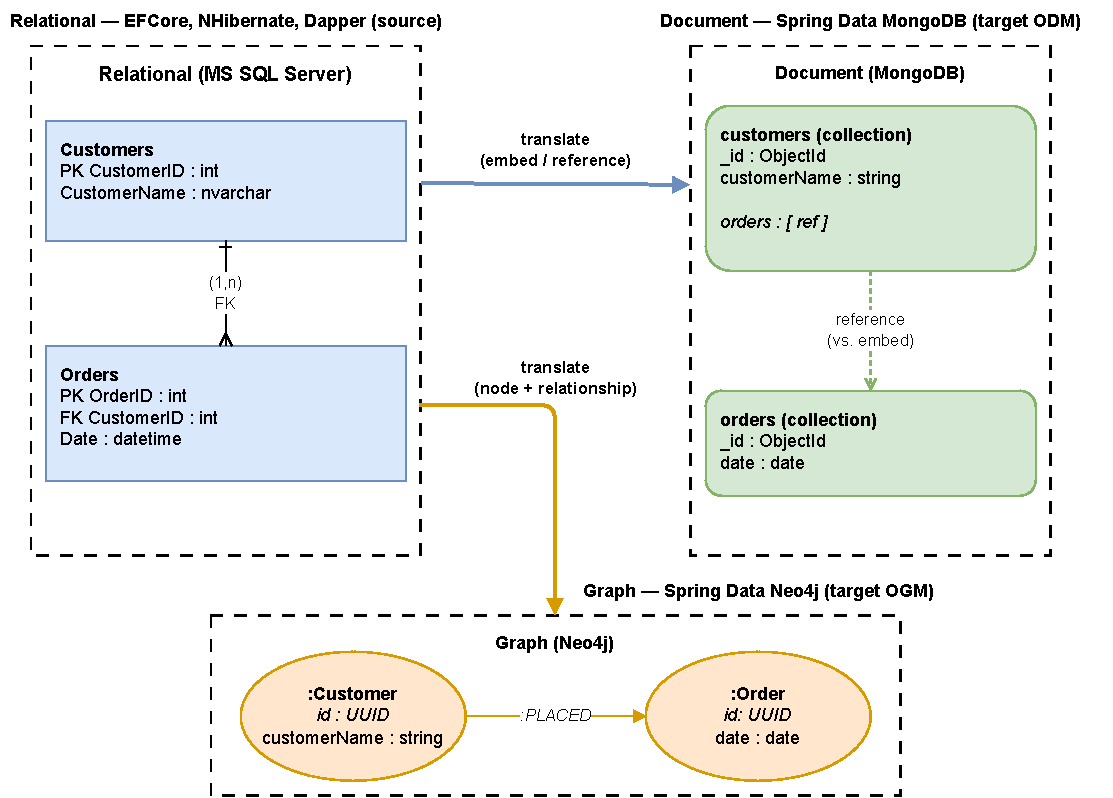
\includegraphics[width=\linewidth]{img/uom_paradigm_mapping.pdf}
\caption{The same relational association translated into the two target models. The document model must choose between embedding and referencing the orders; the graph model turns the entities into nodes joined by a typed relationship.}
\label{fig:paradigm-mapping}
\end{figure} 

Types must be remapped (the integer key becomes a string document identifier). The query must be rewritten into a different idiom (a relational navigation becomes a document aggregation) while returning logically the same result set -- code that merely compiles is not enough. A realistic application multiplies this by dozens of entities and hundreds of queries, each carrying a small decision that can silently break correctness. This is precisely the slow, manual, risky work the assistant is meant to automate \emph{and} verify.

\section{Requirements}
\label{sec:problem-requirements}

The goals of \cref{sec:problem-goals} translate into four properties that a translation produced by the assistant must satisfy. These are the criteria against which the approach is evaluated in \cref{chap:evaluation}.

\begin{description}
  \label{desc:requirements-r1} \item[R1 -- Transformation correctness.] The translated schema and query must be syntactically valid and must compile against the pinned target toolchain. Non-compiling output is rejected before it can reach the user.

  \label{desc:requirements-r2} \item[R2 -- Semantic preservation.] When executed against a live target database holding logically equivalent data, the translated query must return logically the same data as the source query, up to differences that are provably harmless (e.g. field ordering, floating-point precision, or a deterministic reversal of sort order). Equivalence is established by structural comparison of the execution results, not by inspection of the code (\cref{chap:validation}).

  \label{desc:requirements-r3} \item[R3 -- Robustness.] The system must recover from the typical failure modes of language-model code generation -- hallucinated APIs, type mismatches, malformed structured output -- through bounded, automated self-repair, and must degrade gracefully (a controlled hand-off to a human) when repair does not converge.

  \label{desc:requirements-r4} \item[R4 -- Minimal manual intervention.] A correct translation should require as little human effort as possible. The amount of required intervention -- measured as the fraction of runs that reach the human-handoff state -- is a key metric in the evaluation.
\end{description}

Requirements \hyperref[desc:requirements-r1]{R1} and \hyperref[desc:requirements-r2]{R2} are objective, machine-checkable correctness conditions; \hyperref[desc:requirements-r3]{R3} and \hyperref[desc:requirements-r4]{R4} concern the assistant's behaviour around the inevitable cases where the model's first attempt is wrong. The remainder of the thesis shows how the workflow (\cref{chap:workflow}), the orchestration design (\cref{chap:design}), the validation machinery (\cref{chap:validation}), and the prompting strategy (\cref{chap:prompting}) together make these requirements achievable.
